\title{Algebra-Based Physics-1: Midterm 1}
\author{Dr. Jordan Hanson - Whittier College Dept. of Physics and Astronomy}
\date{\today}
\documentclass[10pt]{article}
\usepackage[margin=1.5cm]{geometry}
\usepackage{outlines}
\usepackage{graphicx}
\usepackage{amsmath}
\usepackage{hyperref}

\begin{document}
\twocolumn

\maketitle

\section{Unit 0: Estimation, Unit \\ Analysis, Vectors, and \\ Kinematics I}

\begin{enumerate}
\item Which of the following represents the density of lead?
\begin{itemize}
\item A: 0.11 g cm$^{-3}$
\item B: 1.10 g cm$^{-3}$
\item C: 11.0 g cm$^{-3}$
\item D: 111 g cm$^{-3}$
\end{itemize}
\item A train leaves Los Angeles Union Station for the Bay Area (Emeryville) at 60 km/hr.  If the destination is 600 km to the North, how long before the train reaches the destination?
\begin{itemize}
\item A: 0.50 hours
\item B: 5.00 hours
\item C: 10.0 hours
\item D: 24.0 hours
\end{itemize}
\item What is 25 m s$^{-1}$ in km hr$^{-1}$?
\begin{itemize}
\item A: 15 km hr$^{-1}$
\item B: 25 km hr$^{-1}$
\item C: 60 km hr$^{-1}$
\item D: 90 km hr$^{-1}$
\end{itemize}
\item Suppose a ship accelerates from 0 km hr$^{-1}$ to 10 km hr$^{-1}$ in 60 seconds.  What is the acceleration?
\begin{itemize}
\item A: 60 km hr$^{-1}$ s$^{-1}$
\item B: 6 km hr$^{-1}$ s$^{-1}$
\item C: 1/6 km hr$^{-1}$ s$^{-1}$
\item D: 1/60 km hr$^{-1}$ s$^{-1}$
\end{itemize}
\item Estimate the area of the North Quad of Whittier College (the open space outside the SLC):
\begin{itemize}
\item A: 5000 m$^2$
\item B: 5000 cm$^2$
\item C: 500 m$^2$
\item D: 500 cm$^2$
\end{itemize} \vspace{1cm}
\item A coffee bean is about 0.5 cm$^3$ in volume.  How many could fit in a 2 liter bottle?
\begin{itemize}
\item A: $4\times 10^{1}$
\item B: $4\times 10^{2}$
\item C: $4\times 10^{3}$
\item D: $4\times 10^{4}$
\end{itemize}
\item Let $\vec{v} = v_x \hat{i} + v_y \hat{j}$ represent a velocity vector.  The wind velocity is 10 km/hr, Southwest.  North and East vector components are positive, while South and West are negative.  What are $v_x$ and $v_y$?
\begin{itemize}
\item A: 7.1 and 7.1 km/hr
\item B: -7.1 and 7.1 km/hr
\item C: 7.1 and -7.1 km/hr
\item D: -7.1 and -7.1 km/hr
\end{itemize}
\item What is the angle the velocity makes with the x-axis, in the previous exercise?
\begin{itemize}
\item A: 225 degrees
\item B: 180 degrees
\item C: 135 degrees
\item D: 90 degrees
\end{itemize}
\item (a) Let $\vec{v} = -2\hat{i} + 2\hat{j}$, and $\vec{w} = 2\hat{i} - 2\hat{j}$.  Draw each in a 2D coordinate system below. (b) What is $\vec{v} + \vec{w}$?  (c) What is $\vec{v} - \vec{w}$? (d) Add $\vec{v} + \vec{w}$ and $\vec{v} - \vec{w}$ to your coordinate system. (e) What is $\vec{v} \cdot \vec{w}$? \\ \vspace{2.5cm}
\end{enumerate}

\section{Unit 1: Kinematics II and III}

\begin{enumerate}
\item Suppose a cyclist has a velocity of $15$ m s$^{-1}$ at $t=0$.  If the acceleration is 3 m s$^{-2}$, (a) what is the velocity at $t = 4$ seconds? (b) What is the displacement of the cyclist at $t = 4$ seconds? (c) Are the average and instantaneous velocities different at $t=0$ or $t=4$ seconds?  \\ \vspace{3cm}
\item Consider the motion of the sytem depicted in Fig. \ref{fig:1}.  (a) From the given data, calculate the speed of the system at points P and Q. (b) Is the acceleration of the sytem positive or negative?  Estimate the acceleration. \\ \vspace{3cm}
\item A swan on a lake gets airborne by flapping its wings and running on top of the water. (a) If the swan must reach a velocity of 6.00 m s$^{-1}$ to take off and it accelerates from rest at an average rate of 0.8 m s$^{-2}$, how far will it travel before becoming airborne? (b) How long does this take? \\ \vspace{3cm}
\item \textbf{Design problem}.  Design an experiment in which a baseball is thrown, and the range must be 60 meters.  Choose the launch angle and initial velocity, and show that the range is 60 meters.  Provide the time of flight as well.  Finally, verify your results with the appropriate PhET simulation. \\ \vspace{3cm}
\item \textbf{Design problem.}  In our lab, we used a pendulum to measure $g$, the gravitational constant.  Use the following simulation to repeat that process: \url{https://phet.colorado.edu/en/simulations/pendulum-lab}. Recall that the formula relating period $T$ to $g$ is $T = 2\pi\sqrt{L/g}$, where $L$ is the pendulum length. Show your work in the form of a (handwritten) graph and relevant calculuations. \\ \vspace{4cm}
\end{enumerate}

\begin{figure}
\centering
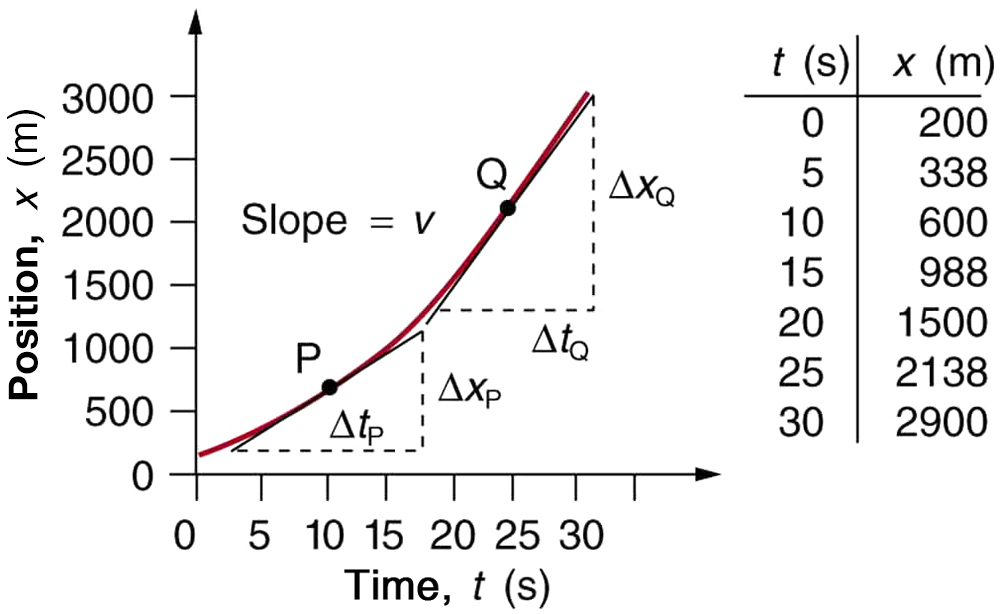
\includegraphics[width=0.4\textwidth]{slope2.jpeg}
\caption{\label{fig:1} A system moves with non-constant velocity.}
\end{figure}

\section{Unit 2: Forces I and II}

\begin{figure}
\centering
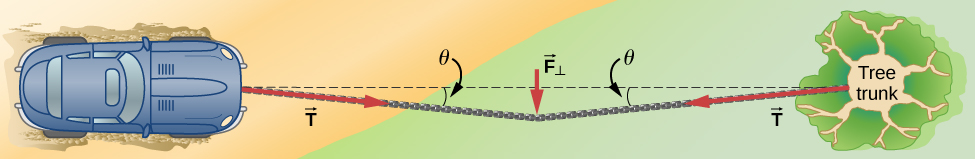
\includegraphics[width=0.5\textwidth]{rope.jpeg}
\caption{\label{fig:2} The net force is zero, just as the vehicle begins to move.}
\end{figure}

\begin{enumerate}
\item Consider the effort to pull a vehicle from a ditch in Fig. \ref{fig:2}. (a) If we can pull with $F_{\perp} = 1000$ N, and observe that the rope makes a 7 degree angle with respect to the line between the vehicle and the tree, what is the tension in the rope? (b) If the vehicle has 900 kg, and the coefficient of kinetic friction is 0.05, what is the acceleration of the vehicle as it starts to move? \\ \vspace{3.5cm}
\item A 20,000 kg jet fighter lands on an aircraft carrier, moving at 120 km/hr. A tow cable grabs the aircraft and pulls it to a stop in 100 meters. (a) What is the average acceleration? (b) What force does the tow cable extert to stop the jet? \\ \vspace{3.5cm}
\item Two children pull a third child on a snow saucer sled exerting forces $\vec{F}_1$ and $\vec{F}_2$ as shown from above in Fig. \ref{fig:3}. Find the acceleration of the 50 kg sled and child system. Note that the direction of friction will be in the opposite direction of the sum of $\vec{F}_1$ and $\vec{F}_2$. \\ \vspace{2cm}
\end{enumerate}

\begin{figure}
\centering
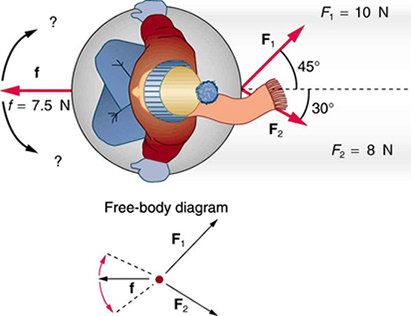
\includegraphics[width=0.33\textwidth]{sled.jpeg}
\caption{\label{fig:3} Two people pull on a third person on a sled, on an icy surface.}
\end{figure}

\section{Unit 3: Forces III and IV}

\begin{figure}
\centering
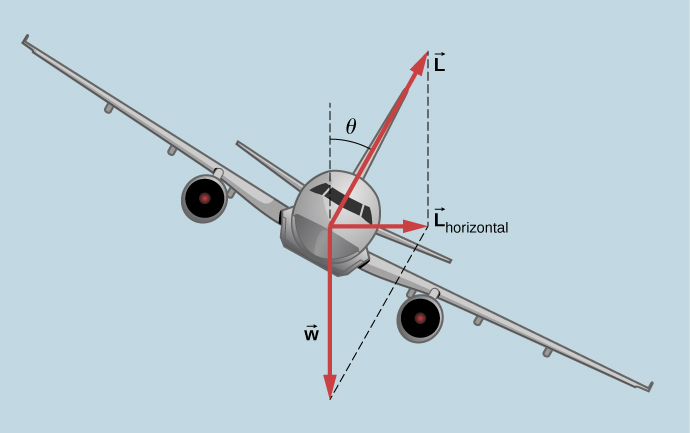
\includegraphics[width=0.45\textwidth]{plane.jpeg}
\caption{\label{fig:4} A plane banks into a circular turn.}
\end{figure}

\begin{enumerate}
\item (a) Show that the acceleration of any object down an incline with friction is $a=g(\sin\theta - \mu\cos\theta)$. (b) What expression do you get as $\mu \to 0$? \\ \vspace{2cm}
\item (a) Use the expression derived in the previous exercise to calculate the acceleration of a snowboarder traveling down a 10 degree incline.  Use the standard values of $g$ and coefficient of kinetic friction between waxed wood and snow. (b) How far down the slope will the person travel after 30 seconds, and what is their speed? \\ \vspace{3cm}
\item Consider Fig \ref{fig:4}, in which a plane flies in a circular trajectory. Suppose the total mass is 6000 kg, $\theta = 30$ degrees, and magnitude of the lift force in Fig. \ref{fig:4} is 80,000 N. (a) What is the centripetal force? (b) If the speed is 600 km hr$^{-1}$, what is the turn radius?  (c) What time will pass before the plane has gone halfway around the circle (to turn around)? \\ \vspace{3cm}
\item Consider three springs connected \textit{in parallel} to an object of mass $m$.  Each spring has a spring constant $k$, and each spring is attached to the floor and the object. (a) Draw a free-body diagram. (b) Derive an expression for the displacement of the springs. (c) Show that, in the limit that $k \to \infty$, the displacement goes to zero.  This is a basic model for the suspension of a vehicle or cart. \\ \vspace{3cm}
\item What is the terminal velocity of a 60 kg skydiver with area $A = 0.25$ m$^2$, and drag coefficient $C = 0.5$?  Use the standard density of air: $\rho = 1.2$ kg m$^{-3}$. (b) What is the terminal velocity if she opens the parachute, increasing the cross-sectional area by a factor of 100? \\ \vspace{3cm}
\item (a) Granite has a standard Young’s modulus of about $45 \times 10^9$ N m$^{-2}$. Calculate the change in length of a granite column supporting 10,000 N of weight.  The column has a diameter of 20 cm, and is 10 meters tall. (b) Suppose the granite column was replaced with a new material with half the Young's modulus.  What would the new change in length be? \\ \vspace{2.5cm}
\end{enumerate}

\end{document}